\documentclass[10pt, a4paper]{article}
\usepackage{sltc2014}
\usepackage{newclude}
\usepackage{graphicx,fixltx2e,dblfloatfix,caption,afterpage}
\usepackage{multicol}

\title{Grammar-based suggestion engine with keyword search}

\name{Martin Agfjord, Krasimir Angelov, Per Fredelius, Svetoslav Marinov} 

\address{University of Gothenburg, Findwise AB\\
               Gothenburg\\ 
               {\tt martin.agfjord@gmail.com, krasimir@chalmers.se}\\ }
\begin{document}

\maketitleabstract

\begin{figure*}[!b]
\centering
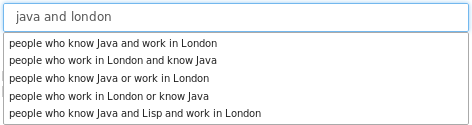
\includegraphics[scale=0.99]{./java-london.png}
\caption{Web interface with suggestions based on the keywords \texttt{java and london} \label{figure}}
\end{figure*}

\section{Introduction}
An alternative approach on building a user friendly interface for a database is  natural language translation. This method has been used before by Facebook \cite{li:2013} in their graph search application, which adopts a grammar to translate structured sentences into machine readable syntax. This paper describes how a similar application can be developed by creating a grammar with \emph{Grammatical Framework (GF)} \cite{ranta:2011} and using \emph{Apache Solr} \cite{kuc:2011} to give relevant suggestions of valid sentences based on keywords or a partial sentence.
\newline
\newline
In order to articulate any sentences we assume this application will be used by a software development company which has a Solr index with the entities \emph{Customers, People} and \emph{Projects}. An example of a valid sentence in this environment is \texttt{people who know Java}, which when executed will instruct the Solr index to retrieve all documents where the field \texttt{object\_type} has the value \texttt{person} and the \texttt{KNOWS}-field contains the value \texttt{Java}. 

While translations like this allows the user to express queries in a natural language, it is not very likely that the user will be able to use the system without any knowledge of the translations it support. We will therefore also develop a suggestion engine which purpose is to help the user to find valid sentences based on partial input.

\section{Grammatical Framework}
GF is an open source development platform for natural languages which is specifically designed for creating natural language grammars. GF adopts the use of abstract and concrete syntax much like compilers do. The abstract syntax represents the \emph{semantics} of a sentence and the concrete syntax represents how the semantics looks like a string in a language. 

An abstract syntax usually consists of unimplemented functions which can be combined to form an abstract syntax tree (AST). A concrete syntax implements the unimplemented functions to represent the semantics as strings. An AST can be \emph{linearized} into a string by executing the functions in a concrete syntax. Conversely, a string can be parsed into an AST by dividing the string into functions.

\section{Defining the grammar in GF}
We define functions to represent \emph{subjects, predicates} and \emph{objects}. In addition, we also define rules which combines these values into sentences. For example, the sentence \texttt{customers who use Solr} is splitted into the AST \texttt{MkInstruction Customer (Use (MkObject "Solr"))} by the grammar. This AST will be linearized into \texttt{select?q=object\_type : Organization AND USES : ( Solr )} by using the concrete syntax for Solr. We make use of arbitrary names in order to let the objects of each sentence take any string.

In addition, we also have functions for boolean operators in the grammar. There are two cases where we allow boolean operators. The first is in between two arbitrary names, e.g. \texttt{Java \textbf{or} Haskell}. The second case is in between two combinations of a predicate and an object, e.g. \texttt{know Java \textbf{and} work in London}. Boolean operators are easily implemented in Solr syntax since it is natural to use them in a query language.

\section{Suggestion Engine}
The grammar can translate sentences from English into Solr query language and offers suggestions of words by using incremental parsing \cite{angelov:2009}. However, suggestion of words can only be used for the next accepted word of a defined partial sentence and can therefore not be used for suggestions on an invalid partial sentence or keywords.

Apache Solr offers functions which approximate how similar a string is to strings stored in a Solr index \cite{kuc:2011}. It makes therefore sense to use Solr to match a partial sentence or only keywords into natural language sentences defined by our grammar.

\subsection{Generation of sentences}
GF offers a \emph{generator} which can generate the AST's a grammar supports. We generate all AST's up to a certain limit. The limitation is needed as we have infinitely many AST's because of the recursive boolean functions. Since we use arbitrary strings in our grammar, GF will use  \texttt{"Foo"} in an AST when it expects a name. We will therefore generate AST's like \texttt{MkInstruction People (WorkIn (MkObject "Foo"))} which linearizes into \texttt{people who work in Foo}. This linearization would not be very helpful as a suggestion to a user since \texttt{Foo} is not a location.

A solution is to replace \texttt{Foo} with a relevant name before presenting the suggestions to a user (we assume all names exists in a separate Solr index). However, as we treat all names as objects, it would be possible for suggest many strange sentences to the user, such as \texttt{people who work in Haskell}.

In order to make distinctions between different names we introduce \emph{name types}. A \texttt{Skill} is a programming language, an \texttt{Organization} is an organization, a \texttt{Location} is a physical location and a \texttt{Module} is an application module. The previous AST now looks like this \texttt{MkInstruction People (WorkIn (MkLocation "Foo"))}. The function \texttt{MkLocation} reveals that the name in this function is of the type \texttt{Location}. 

The English linearization of the previous AST will however still not contain anything about the type, since the linearization of the AST \texttt{MkSkill "Foo"} is \texttt{Foo}. To preserve the type of each name, we post-process each AST and replace \texttt{"Foo"} with the actual type and an index, in this example \texttt{"Location"}.

\subsection{Suggestion retrieval}
 We generate sentences as described in the previous section and store them in a Solr index. This section describes how we take an input from the user and present relevant suggestions based on the input. This method is rather na\"{\i}ve and can definitely be better.

 We split an input on words and check if each word is a name by asking the Solr index which contains all names (and their types). If a word is a name, we replace it in the input with its type plus an index. For example, the sentence \texttt{people java} will be changed into \texttt{people Skill0}. We fetch the five most similar sentences from the Solr index by using Solr's query interface. In this example, the first result is the sentence \texttt{people who know Skill0}. Finally, we change back Skill0 into \texttt{Java} in each sentence.

\section{Conclusions}
The results from Agfjord, 2014 show that this method of building a natural language interface provides makes it possible to translate from natural languages into a query language. We do not see any limitation to only query languages, rather, any machine readable language could be used in place of Solr query language.

We found out it was easy to develop a translating service by using GF. It is also easy to extend the grammar to support translation of more sentences. In addition, it was simple to map \emph{ungrammatical} sentences into grammatically correct sentences. This made the suggestion engine more powerful.

The suggestion engine is fast and scalable, as the Solr index only need to store one sentence per AST for each natural language. This is possible since we only use name types in the sentences and not actual names. A user can find relevant defined sentences by using only keywords. If a keyword is a name, then the application will recognize the type of the name and correctly use it with defined sentences.

However, there are still some functionality left to implement in the suggestion engine. One thing is heuristic on which names that are relevant if no names exists in the input. Another improvement is to remove sentences with the same meaning as another sentence in the index. An example can be seen in Figure 1 where suggestion 1 and 2 has the same meaning but however does not share the same AST.

The suggestion engine can be used together with speech recognition software. One first translate speech into a string, which is passed to the suggestion engine. Speech strings are often not exactly correct, but this is not an issue as we map the input to the most relevant sentence. In addition, since Solr has built in string approximation functions, we can use them on individual words to allow misspelled or similar words to represent defined words in sentences.

By realizing speech to machine readable syntax translation we open up doors to many new applications such as interfaces for cars and other devices which has limited keyboard interaction.

\bibliographystyle{sltc2014}
%\bibliography{sltc2014} 
\include*{bibliography}
\end{document}
